\documentclass[8pt]{beamer}
\usepackage{lmodern} % font
\usetheme{Marburg}
%\usecolortheme{albatross} %Nice but figures need to be produced accordingly
%\setbeamertemplate{headline}{}
\setbeamertemplate{navigation symbols}{}

\usepackage{tikz}
\tikzset{>=latex}
\usetikzlibrary{calc, arrows, decorations.markings}

\definecolor{sblue}{RGB}{76, 114, 176}
\definecolor{sorange}{RGB}{221, 132, 82}
\definecolor{sgreen}{RGB}{85, 168, 104}
\definecolor{sred}{RGB}{196, 78, 82}
\definecolor{spurple}{RGB}{129, 114, 179}
\definecolor{sbrown}{RGB}{147, 120, 96}
\definecolor{spink}{RGB}{218, 139, 195}
\definecolor{sgray}{RGB}{140, 140, 140}
\definecolor{syellow}{RGB}{204, 185, 116}
\definecolor{scyan}{RGB}{100, 181, 205}


\title{Benchmarking of modcell-hpc for large scale problems}
\subtitle{Research report}
\author{Sergio Garcia}

\begin{document}
\begin{frame}
\titlepage
\end{frame}

\section{Implementation}
\begin{frame}{Brief description of implementation}

        \begin{itemize}
            \item The Matlab implementation of ModCell2 is slow and cannot handle large-scale problems due to both its inability to effectively parallelize beyond a few cores and its inefficient use of CPU and memory resources.
                \item modcell-hpc was written from the bottom up in C and uses MPI to implement island parallelization. In this approach multiple instances of the algorithm run in individual processes known as islands. These islands exchange individuals with certain periodicity in a process called migration.
    \end{itemize}

\begin{figure}[H]
    \centering
    %\fbox{\includegraphics[keepaspectratio, width=\textwidth]{./combined.png}}

\tikzset{font=\large}
\resizebox{0.3\textwidth}{0.3\textheight}{%
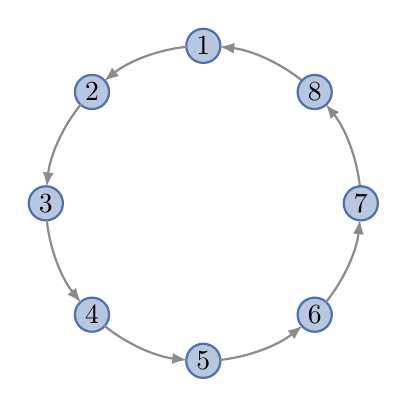
\begin{tikzpicture}[
    island/.style={circle,draw=sblue,fill=sblue!40,thick,inner sep=1.5pt,minimum size=6pt}
  ]

  \node (center) at (0,0) {};

    \def \n {8}
    \def \radius {2}
    \def \margin {6}

    \foreach \s in {1,...,\n} {
        \node[island] (c\s) at ($(center) + ({360/\n * (\s + 1)}:\radius)$) {\s};
        \draw[->,thick,sgray] ($(center) +({360/\n * (\s - 1)+\margin}:\radius)$)
        arc ({360/\n * (\s - 1)+\margin}:{360/\n * (\s)-\margin}:\radius);
    }


\end{tikzpicture}}
    \caption{Islands with 8 processors in ring topology.}
\end{figure}

        \begin{itemize}
                \item Migration occurs asynchronously so islands may continue to evolve while messages are being passed, greatly enhancing performance.
                \item This approach can potentially scale to hundredths or thousands of cores since the program does not contain any sequential operations that would become a bottleneck (See Amdahl's Law).
    \end{itemize}

\end{frame}

\section{Reproduce previous results}
    \begin{frame}{Reproduce previous results}
        \begin{itemize}
            \item Garcia and Trinh Metabolic Engineering 2019: \textit{E. coli} model 20 products, wGCP-4-0. In a single run, 32 non-dominated solutions were found, including the target solution compatible with 17 products. In several runs, a total of 701 solutions were found, with 5 of them having a compatibility (threshold 0.6) of 17:
        \end{itemize}

        \vspace{0.5cm}
        \centering
        \begin{tabular}{l|l}
            Solution index &	Deletion ID\\
            \hline
            66	& ACALD, PTAr, TKT2, LDH\_D \\
            202	& ACALD, PTAr, GND, LDH\_D \\
            187	& ACALD, TKT1, PTAr, LDH\_D\\
            125	& ACALD, PGL, PTAr, LDH\_D\\
        \end{tabular}

    \end{frame}

\section{Benchmark}
\subsection{Parameters and metrics}
\begin{frame}{Parameters and metrics}

    Parameters under consideration for stage 1 (20 products):
\begin{itemize}
    \item Population size: Number of individuals per island.
    \item Migration type: 1) ReplaceBottom, top individuals are sent and bottom individuals are replaced. 2) Random, random individuals are sent and replaced.

    \item Migration interval: Number of generations between migration events.
\end{itemize}
    Parameters under consideration for stage 2 ($>100$ products):
\begin{itemize}
    \item Run time: Fixed run time for which the problem runs.
    \item Number of cores: Number of cores that corresponds to the number of islands
\end{itemize}
    Metrics:
\begin{itemize}
    \item Coverage: Fraction of points from all Pareto optimal solutions found captured by a given parameter configuration. Only unique Pareto points are taken and thus alternative solutions are not taken into account.
    %\item $GD$ and $\Delta P$: These are averages of euclidean distances between found solutions and the reference Pareto front.
    \item Smallest number of designs that cover all compatible products. Note that if only a few products are compatible this can lead to smaller cover sizes, so the same number of products should be compatible to compare this value.
\end{itemize}
\end{frame}

\subsection{Stage 1: 20 products}

\begin{frame}{\protect\textit{E. coli} and 20 products: Results}

These simulations were conducted on ACF with 16 processes each and design parameters $\alpha=6,\beta=1$.

\begin{figure}
    \centering
    \includegraphics[keepaspectratio, width=1.05\textwidth]{raw/gem-model.png}
    %\caption{$\alpha=6,\beta=1$, 1 hour run time.}
\end{figure}
\end{frame}

\begin{frame}{\protect\textit{E. coli} and 20 products: Conclusions}
Findings:
\begin{itemize}
    \item For limited run time, smaller populations go through more generations and achieve better results. Thus when run time is fixed, instead of generations as in the MOEA comparison paper, an optimal population size can be found.
    \item The effect of the migration frequency is tied to the number of generations, which is affected by the population size.
    \item The ReplaceBottom migration policy is better than random.
\end{itemize}
    Conclusion:
\begin{itemize}
    \item The ReplaceBottom migration policy will be selected.
    \item A migration frequency of 25 will be selected.
    \item Different population sizes will be tested for the larger problem to determine a good value.
\end{itemize}

\end{frame}

\subsection{Stage 2: 161 products}
\begin{frame}{\protect\textit{E. coli} and 161 products: Results}

\begin{figure}
    \centering
    \includegraphics[keepaspectratio, height=0.93\textheight]{raw/native.png}
    %\caption{\a}
\end{figure}
\end{frame}

\begin{frame}{\protect\textit{E. coli} and 161 products: Conclusions}

    Findings:
\begin{itemize}
    \item At 5h a population size of 200 is better in all metrics. While at 10h 200 and 300 are more similar. This indicates that the population size of 100 is too small, and that after a given number of generations populations sizes of 200 and 300 are comparable. So we will use 200 as the smallest valid population size per island.
    \item Increasing the number of cores leads to more solutions, but this does not mean those solutions are necessary better in terms of minimal covers. There is a trade-off in communication as the number of cores increases, which could affect overall convergence of the meta-population. This could be addressed with different topologies (e.g., hypercube) but that is currently beyond the scope of this study.
    \item In both cases around 48 cores reach a plateau in terms of compatible modules and cover size.
\end{itemize}


    Conclusions:
\begin{itemize}
    \item A population size of 200 is the minimum required for proper convergence and should be used under limited run times.
    \item 48 cores will be used for future studies.
\end{itemize}
\end{frame}

\end{document}


